\documentclass{beamer}
\usepackage{graphicx}
\author{Peter Davoust \& Nicolas Langley}
\title{Automatic Panoramic Image Stitching}
\usetheme{default}

\begin{document}

\begin{frame}[plain]
	\titlepage
\end{frame}

\begin{frame}{Example}
	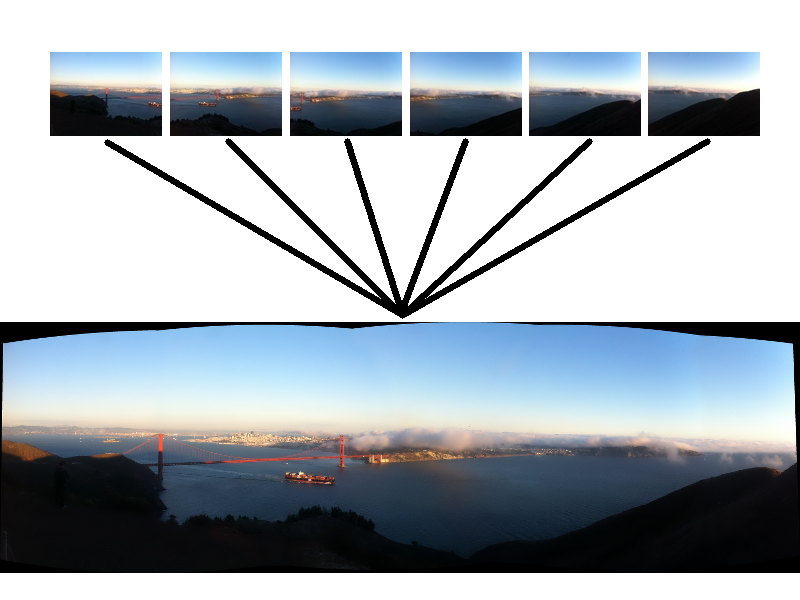
\includegraphics[width=\textwidth]{StitchExample.png}
\end{frame}

\begin{frame}{Problem Definition}
	\begin{itemize}
		\item Given an unsorted collection of images
		\begin{itemize}
			\item Images may or may \emph{not} fit together
		\end{itemize}
		\item Find corresponding points in the collection of images
		\item Determine whether or not correspondences are valid
		\item Align images properly
		\item Warp images so corresponding points overlap
		\item Correct gain
	\end{itemize}
\end{frame}

\begin{frame}{Finding Correspondences}
        \begin{itemize}
            \item In order to find correspondences between images, a homography for each image must be estimated
            \item This can be done in two different ways
            	\begin{enumerate}
			\item Direct: search for alignments of given images that minimizes the differences between overlapping \
					 images. Typically require initialization by the user and give a very accurate representation due \
					 to using all available image data.
			\item Feature-Based: involves identifying features within each image and then aligning images based on \
					 occurrences of matching features
		\end{enumerate}
	   \item We are focusing on feature-based matching using SIFT (Scale-invariant feature transform) features to characterize our images. This allows for us to handle images with varying orientation and zoom.
        \end{itemize}
\end{frame}

\begin{frame}{Validity of a Correspondance}
        \begin{itemize}
            \item In order to properly match images and align them to form a panorama it is important to verify that the image matches found using image features are accurate and valid.
            \item For each pair of matched images, a probabilistic model can be employed to verify that the match is correct.
            \item This process involves computing the probabilities that the set of geometrically consistent feature matches and feature matches that occur in an area of overlap but are not consistent were generated by a correct image match or a false image match.
            \item Once pairwise matches between the images have been verified, panoramic sequences can be expressed as connected sets of matching images.
        \end{itemize}
\end{frame}

\begin{frame}{Alignment with Bundle Adjustment}
	\begin{itemize}
		\item Matching homographies would lead to issues
		\item Not all images would align
		\item Bundle adjustment [TMHF99] solves this problem
	\end{itemize}
	\begin{figure}[H]
	\centering
	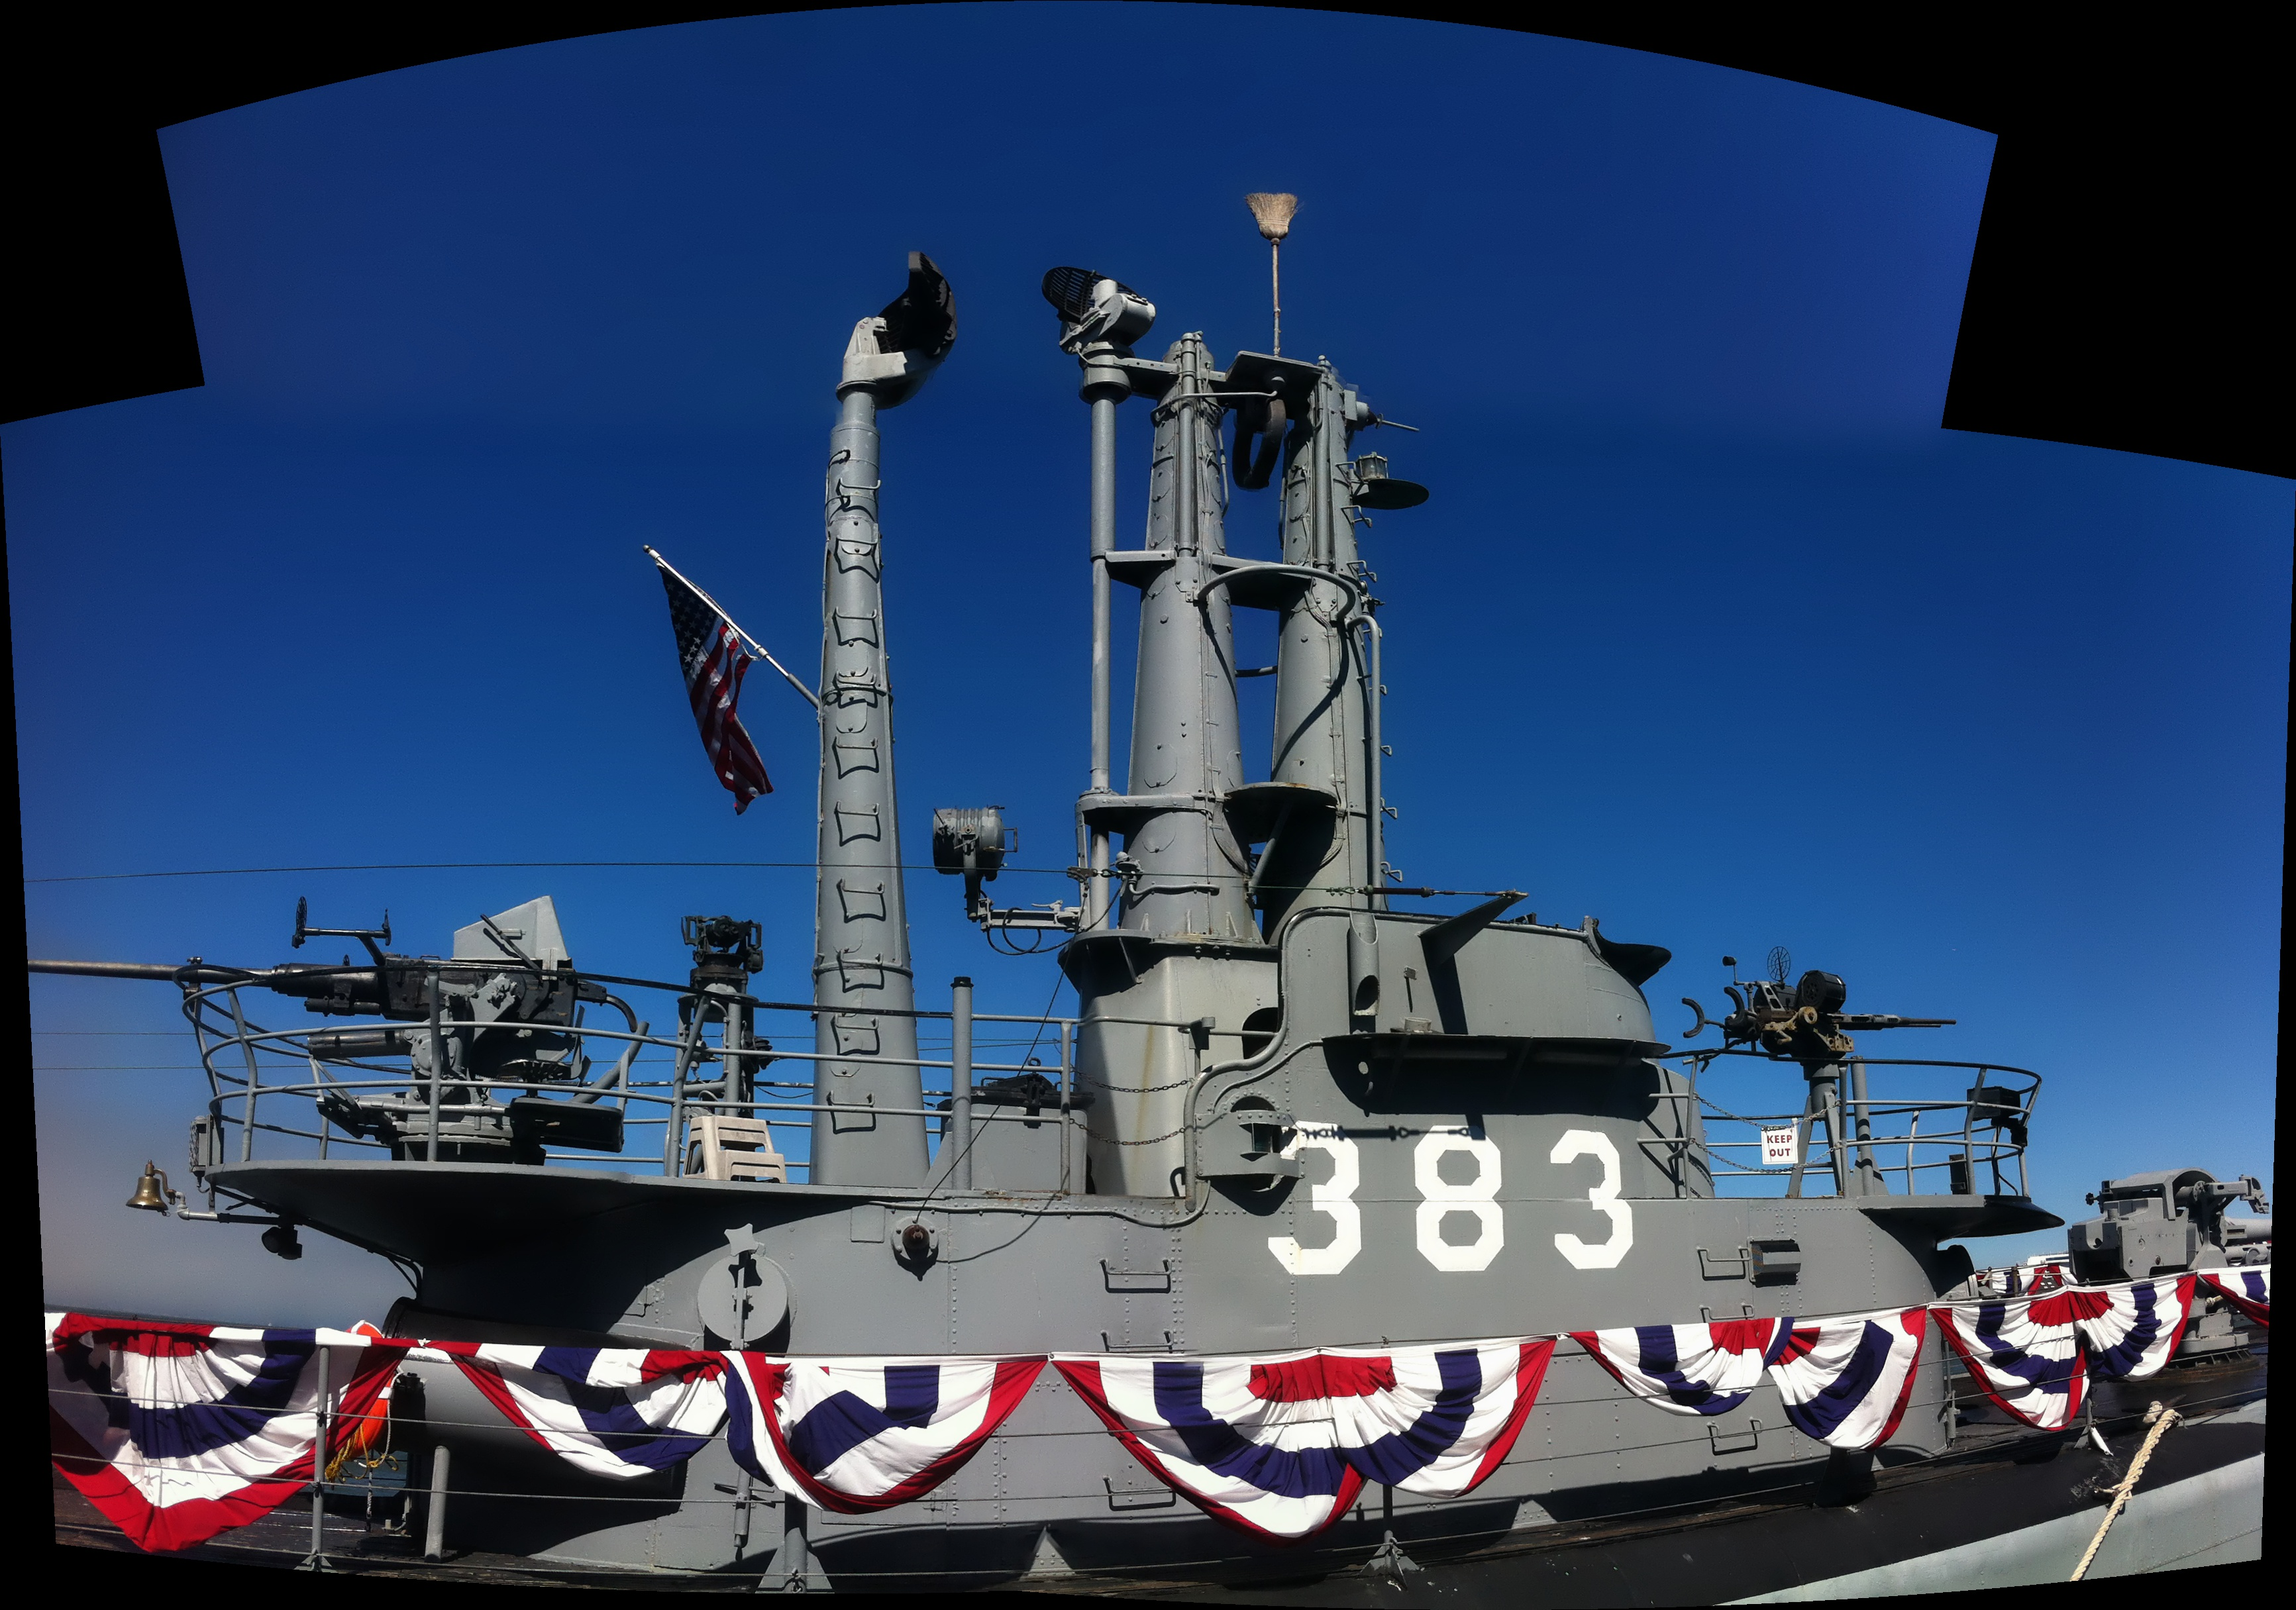
\includegraphics[width=0.7\textwidth]{Sub.jpg}
	\end{figure}
\end{frame}

\begin{frame}{Straightening}
	\begin{itemize}
		\item The resulting panorama may not be perfectly level
		\item Cameras are not perfectly level
		\item Assume camera is level relative to the horizon
		\item Straighten so the null space of the covariance of the horizontal axis is up
	\end{itemize}
\end{frame}

\begin{frame}{Gain Correction}
\begin{itemize}
	\item Modern consumer cameras adjust gain automatically from image to image
	\item Variation of lighting conditions over an image may necessitate changes in exposure and aperture settings across the panorama
	\item Minimize the gain normalized intensity error over all overlapping pixels ($\mathcal{R}(i,j)$)
	\item Solve for the gain parameters $g_i, g_j$.
\end{itemize}
\begin{align}
e = \frac{1}{2} \sum^n_{i=1} \sum^n_{j=1} |\mathcal{R}(i,j)| \Big(\frac{(g_i \bar{I}_{ij} - g_j \bar{I}_{ji})^2}{\sigma_N^2} + \frac{(1-g_i)^2}{\sigma_g^2}\Big)\\
\bar{I}_{ij} = \frac{\sum_{u_i \in \mathcal{R}(i,j)} I_i(u_i)}{\sum_{u_i \in \mathcal{R}(i,j)} 1}
\end{align}

\end{frame}

\begin{frame}{References}
\begin{itemize}
\item W. Triggs, P. McLauchlan, R. Hartley, and A. Fitzgibbon. Bundle adjustment: A modern synthesis. In Vision Algorithms: Theory and Practice, number 1883 in LNCS, pages 298– 373. Springer-Verlag, Corfu, Greece, September 1999.
\item M. Brown and D. Lowe. Automatic Panorama Stitching using Invariant Features. IJCV, 2007.
\end{itemize}
\end{frame}

\end{document}
